%!TEX root=../book.tex

\chapter{Correlation}

\section{Overview of Correlation}

\subsection{Scatterplots}
Okay, so this is something that we could have presented back a few chapters ago when we talked about data visualization. Unfortunately, that wouldn't have worked with the example we were using, so instead of completely switching gears on you, we decided to wait until now to present it.

Scatterplots \index{Scatterplot} are used to display data using cartesian coordinates. For instance, we may wish to visualize the growth of the U.S. population by decade (Figure \ref{fig:correlation01}).

\begin{figure}[htp]
	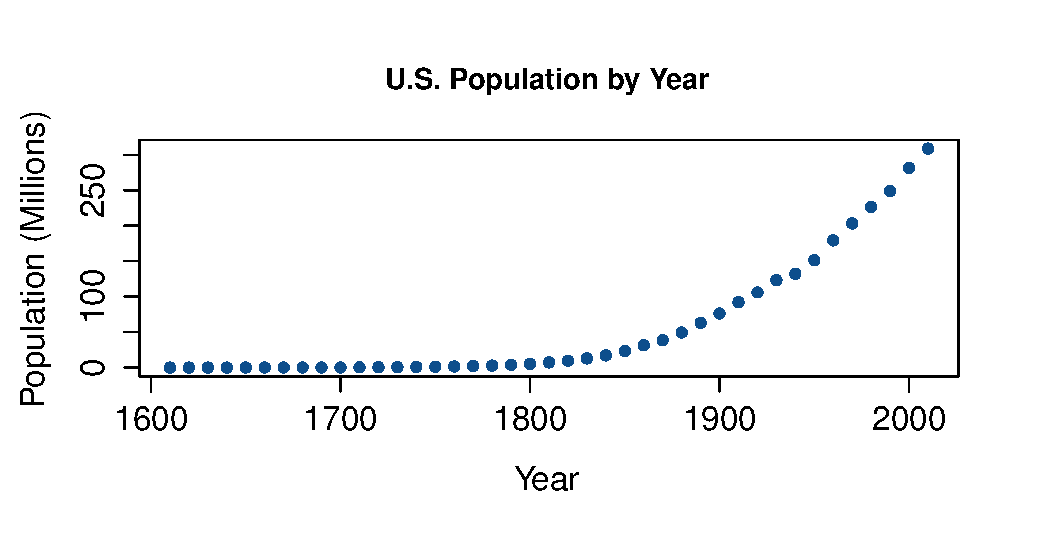
\includegraphics[width=\textwidth]{correlation01}
	\caption{United States population by decade: 1600 through 2010}
	\label{fig:correlation01}
\end{figure}

\subsubsection{Scatterplots with Categorical Variables}
Additionally, we can use scatterplots to visualize data with categorical indicators. For example, if we were interested in the depression and anxiety scores of patients with mild, moderate, and severe bipolar diagnoses (Figure \ref{fig:correlation02}).

\begin{figure}[htp]
	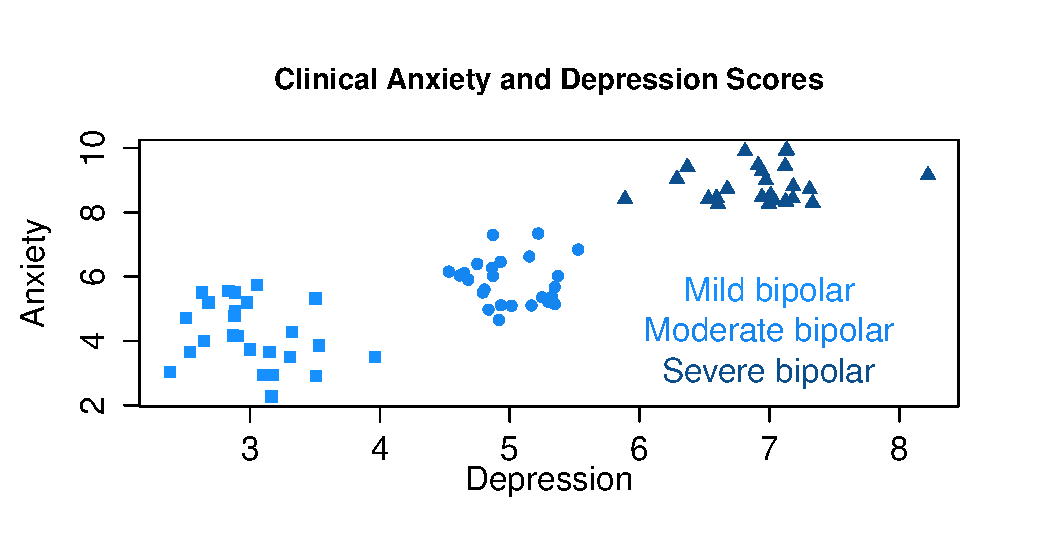
\includegraphics[width=\textwidth]{correlation02}
	\caption{Depression and anxiety scores of patients with bipolar depression}
	\label{fig:correlation02}
\end{figure}

\subsection{Correlation: Measuring Linear Association}
Woah, hold up now: measuring linear association \index{Linear association}? This sounds like we're heading towards some scary waters. Linear association? I thought this wasn't supposed to be a mathy book!

Don't worry, we didn't lie to you. That's just a bit of a scary term for a not-so-scary concept. \textbf{Linear association}, in its most basic form, just means that when you increase one variable by so many units, another variable increases by so many other units. For instance, let's say that for every degree Fahrenheit we increase, we increase the number of daily neighborhood ice cream sales by 10 cones. That's easy, right?

And that's all that correlation \index{Correlation} is measuring: the degree to which a change in one variable coincides with a change in another variable. Now, importantly, this doesn't mean that one causes the other. As a matter of fact, that's so important that it gets its own section a little ways down the page. But, as long as we keep that in the back of our minds for now, we can go ahead and define correlation as:

\begin{eqnarray}
\rho_{X,Y} =& \frac{\text{cov}(X,Y)}{\sigma_X\sigma_Y} &\text{ for a population} \\
r=& \frac{1}{n-1}\sum_{i=1}^n\left(\frac{x_i-\bar{x}}{s_x}\right)\left(\frac{y_i-\bar{y}}{s_y}\right) &\text{ for a sample}
\end{eqnarray}

So, although this looks like we're going back into the Forbidden Forest, it's a pretty straightforward couple of equations: they're saying that this correlation coefficient $r$ is just equal to the covariance of two variables, $x$ and $y$, divided by the product of their standard deviations. Or, put another way, it's the amount that two variables change together divided by the amount of that change that we can attribute to chance.

This will then give us a single value, $r$, which can be anywhere from -1 to +1. Now, in this case, both negative and positive 1 mean the same thing (or pretty close to the same thing): this coefficient tells us about the strength of the relationship between the two variables. So, if we have $r=-1$, that means that for every increase of $x$ units of one variable, we decrease by $y$ units of a second variable. Likewise, for $r=1$, this tells us that for every $x$ units that we increase one variable, we increase the other by exactly $y$ units. Finally, if we have $r=0$, that tells us that there is absolutely no relationship between our two variables. In other words, you could increase one variable by over 9000 units and absolutely nothing would change in your second variable.

Unfortunately, most of us will never see a correlation that strong in real life: that would mean that there is absolutely no variance of your data. Now, if we're talking about a physical law and measuring it with incredibly high-precision instruments, it's entirely possible that we will have a correlation that strong. However, in most studies, there will be some random variance thrown in that weakens the correlation.

So remember:

\begin{eqnarray*}
r=& \pm1 &\implies \text{strong correlation} \\
r=& 0 &\implies \text{weak correlation}
\end{eqnarray*}


\subsection{Correlation Matrices and Multiple Correlation}
We know that correlation is a measure of dependence between two variables. However, there may be times when you want to examine multiple variables at once. In cases like this, it may be useful to create a \textbf{correlation matrix} \index{Correlation matrix}. This is simply a lower-triangular matrix of correlations among multiple variables.

For instance, let's say that we want to see how adiposity in different parts of the body correlate. We may do something like:

\begin{framed}
\begin{Verbatim}[samepage=TRUE]
as.dist(cor(bodyFat))

          Neck    Chest   Abdomen  Hip
        +-------------------------------
  Chest | 0.766 
Abdomen | 0.728   0.911
    Hip | 0.705   0.823   0.860  
  Thigh | 0.668   0.708   0.736    0.881
\end{Verbatim}
\end{framed}

Here we can see the correlations between Neck, Chest, Abdomen, Hip, and Thigh adiposity---ranging from 0.67 to 0.91. However, what if we wanted to visualize these correlations as scatterplots? We might generate a lower-triangular scatterplot matrix using the \verb|pairs()| function (Figure \ref{fig:correlation03}):

\begin{framed}
\begin{Verbatim}[samepage=TRUE]
pairs(~Neck+Chest+Abdomen+Hip+Thigh,
    data=bodyFat,upper.panel=NULL)
\end{Verbatim}
\end{framed}

\begin{figure}[htp]
	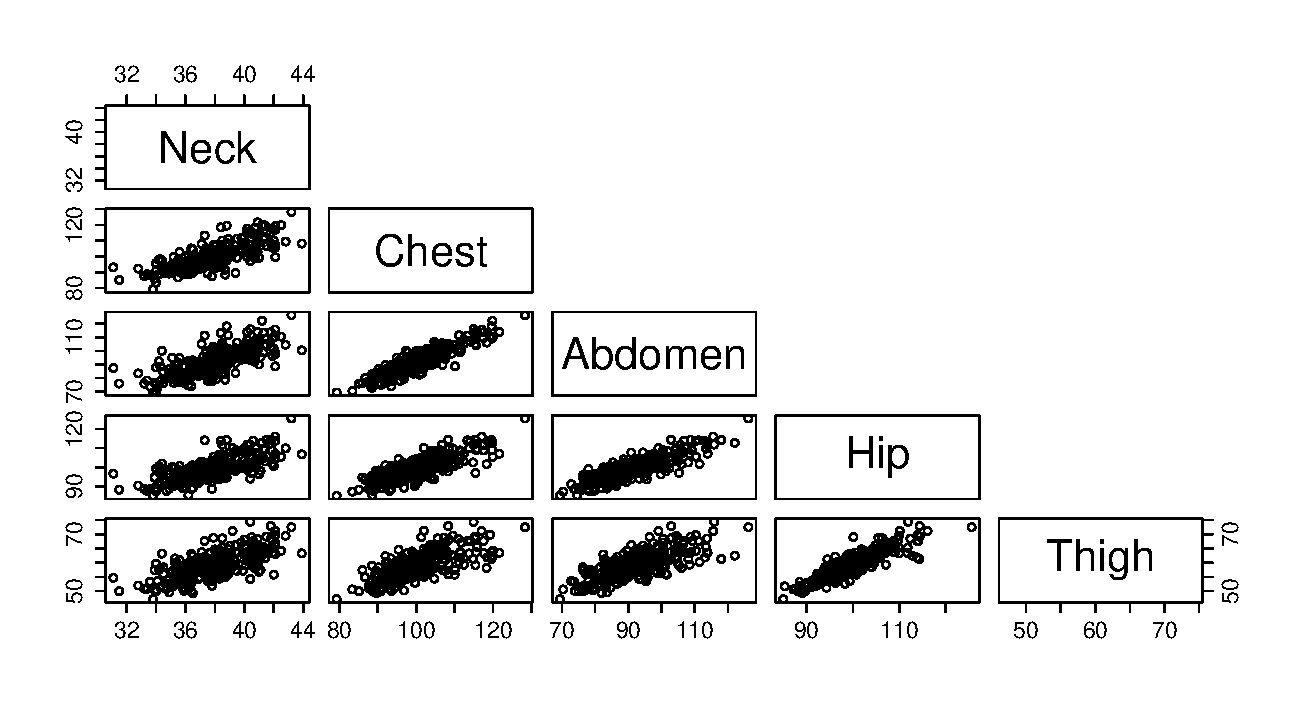
\includegraphics[width=\textwidth]{correlation03}
	\caption{Lower-triangular scatterplot matrix for multiple correlations}
	\label{fig:correlation03}
\end{figure}

Finally, we will likely want to assess the significance of these correlations. To do so, we will have to install the Hmisc package:

\begin{framed}
\begin{Verbatim}[samepage=TRUE]
install.packages("Hmisc")
library(Hmisc)
rcorr(as.matrix(bodyFat))
\end{Verbatim}
\end{framed}

This will return all bivariate correlations \index{Correlation!Bivariate correlation} and levels of significance for the specified matrix. (NB: The data must be input as a matrix for this function to work. If you are using a data frame, first pass it through the \verb|as.matrix()| function.)

\subsection{Partial Correlations}
In our previous section, we looked at correlations among multiple variables. These were all referred to as \textbf{bivariate correlations} because each correlation only looked at exactly two variables. However, we saw that each of those 5 variables correlated significantly with each of the others. So it may be more appropriate to conduct a \textbf{partial correlation} \index{Correlation!Partial correlation}: this will take two variables---say, Neck and Chest---and measure their degree of association after controlling for the effect of Abdomen, Hip, and Thigh. This approach is generally preferred if there are other known sources of covariance that you also measured.

\section{Cautions and Considerations}
\subsection{Causal Inferences}
Importantly, one cannot make causal inferences from correlational designs: if you think back to the chapter on research design, for a causal inference to by justified, there must be (1) temporal precedence; (2) covariation; and (3) nonspuriousness. Here, we violate the first and third assumptions. Regarding temporal precedence, neither of the measures that we are looking at clearly precedes the other: the measurements could be made simultaneously; one could always occur before the other; or the order of occurrence could be random at each point of measurement. Additionally, correlational studies don't have any control or experimental conditions in place to ensure that potential confounding variables are controlled for and don't give rise to spurious correlations.

Given these concerns, we are only able to say that Variable A and Variable B tend to covary: that is, when one changes in a certain way, the other is likely to change in a certain way. For instance, consider height and weight. Let's say that there is a positive correlation between the two (i.e., that taller people tend to weigh more and that people who weigh less tend to be shorter). We can say that someone who is 6'1" is likely to weigh more than someone who is 4'10"; however, it becomes silly to say that if someone loses weight, he or she will start shrinking in height. Likewise, by gaining weight, no one will ever grow taller. There is a general trend of the data; however, this does not mean that a change in one ever causes a change in the other.

\subsection{Linearity of the Relationship}
Another consideration when looking at correlations is the relationship between the two variables of interest. Namely, there must be a linear trend. In this context, a linear trend is going to mean that every time Variable A changes by $x$ units, Variable B will change by $y$ units. For instance, take the four plots in Figure \ref{fig:correlation04}.

\begin{figure}[htp]
	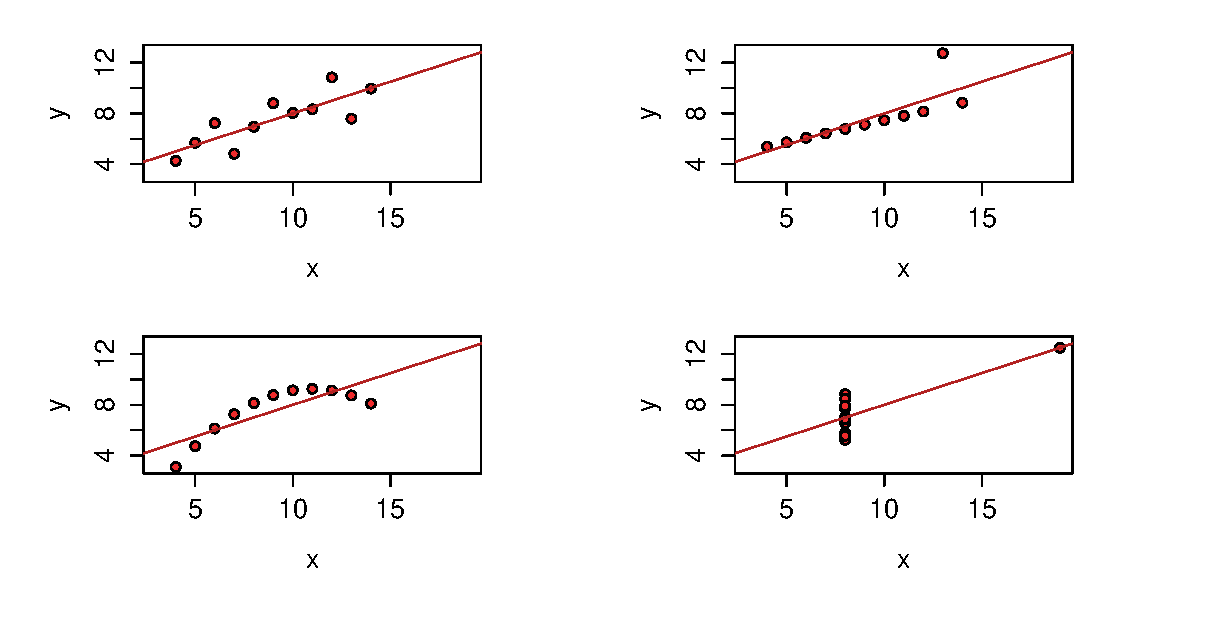
\includegraphics[width=\textwidth]{correlation04}
	\caption{Four separate data sets, each with the same mean and correlation. Source: \href{http://en.wikipedia.org/wiki/Correlation}{Wikipedia}}
	\label{fig:correlation04}
\end{figure}

Here we have four different relationships between our two variables with the same regression line plotted against all of them. As far as a correlation is concerned, the data follow that solid line.

\subsection{Sensitivity to the Distribution}
Also important is the distribution of the data. Although the degree of dependence between two variables $X$ and $Y$ is unaffected by transformations of the data where both $X$ and $Y$ are transformed by constants, the strength of correlation is highly impacted by the range of values sampled. Generally, the wider the range that is sampled, the stronger the correlation will be between the two measures.

Take, for instance, Figure \ref{fig:correlation06}. In orange are the unrestricted data, giving a correlation of $r=0.897$. Yet, when we restrict our range to only values of $X$ on the interval $(0,1)$, that correlation drops to $r=0.387$ although no transformations or other alterations were made to the data. Given these concerns, there have been attempts to correct for this range restriction; however we will not detail them here. Generally, this is not often a major issue to researchers; however, if you know that your data will be somehow restricted, it is good to keep in mind that this may impact the correlation coefficient.

\begin{figure}[htp]
	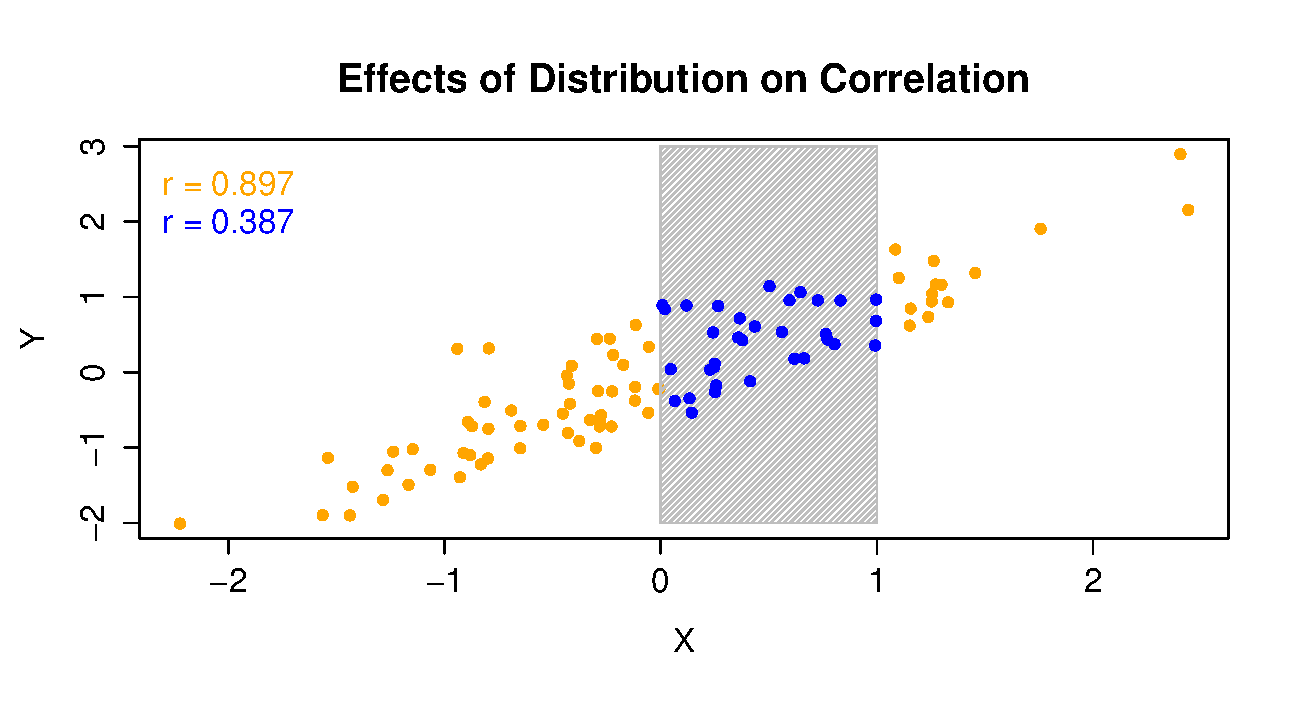
\includegraphics[width=\textwidth]{correlation06}
	\caption{Pearson correlation coefficients between X and Y are shown when the two variables' ranges are unrestricted (orange) and when the range of X is restricted to the interval (0,1) (blue)}
	\label{fig:correlation06}
\end{figure}

\section{Implementation in R}

\subsection{Correlation}
Using R, if we want to look at the correlation between two variables, we can do so using the \verb|cor()| function. Alternately, if we want to see if there is a \textbf{significant} correlation between those two variables, we use the \verb|cor.test()| function. For instance, if we wished to see the correlation between amounts of neck and chest fat, we would run:

\begin{framed}
\begin{Verbatim}[samepage=TRUE]
cor.test(bodyFat$Neck, bodyFat$Chest)

	Pearson's product-moment correlation

data:  bodyFat$Neck and bodyFat$Chest
t = 18.7782, df = 247, p-value < 2.2e-16
alternative hypothesis: true correlation is not equal to 0
95 percent confidence interval:
 0.7102541 0.8136117
sample estimates:
      cor 
0.7668596 
\end{Verbatim}
\end{framed}

As we can see, there was a correlation between the two variables of $r=0.77$ and this reached a level of statistical significance, $t = 18.78$; $p\text{-value}<0.001$. Because our $p$-value was below the $0.05$ threshold, we can conclude that the relationship between the two variables actually exists. This means that individuals with more neck fat tend to also have more chest fat, and vice versa.

\subsection{Partial Correlation}

To run a partial correlation in R, we will execute something like:

\begin{framed}
\begin{Verbatim}[samepage=TRUE]
source("http://www.yilab.gatech.edu/pcor.R")

neck <- bodyFat$Neck
chest <- bodyFat$Chest
others <- subset(bodyFat, select=c(Abdomen:Thigh))

pcor.test(neck,chest,others)

   estimate  p.value  statistic
  0.344  9.7e-09   5.73  249
\end{Verbatim}
\end{framed}

We can see that the observed correlation drops from $r=0.766$ with the bivariate correlation to $r=0.344$ with the partial correlation. This means that, when we control for the effects of Abdomen, Hip, and Thigh adiposity, neck and chest still covary significantly with a correlation of about 0.34.

\section{Case Study: National Education Trends}

These data are taken from the Census' American Community Survey. Here, we have two columns that we're interested in: \verb|highSchoolorHigher| and \verb|perCapitaIncome|. We would like to see if there is a relation between a state's per capita income and the proportion of its residents to have completed high school or higher. So let's start by constructing a scatterplot of the two variables, seen in Figure \ref{fig:correlation05}:

\begin{figure}[htp]
	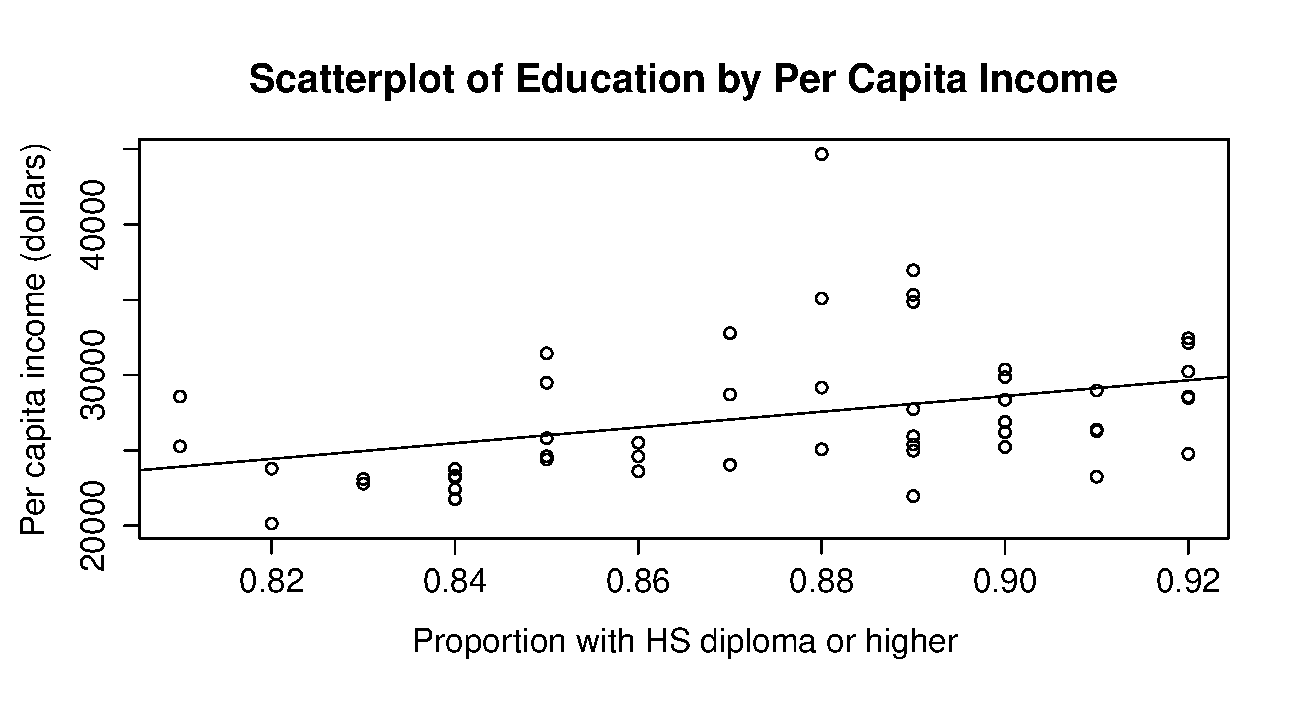
\includegraphics[width=\textwidth]{correlation05}
	\caption{Scatterplot of perCapitaIncome and HighSchoolOrHigher}
	\label{fig:correlation05}
\end{figure}

As we can see, there appears to be a positive linear relationship between per capita income and the proportion of a state's residents having a high school diploma or higher. Our next step is then to quantify the strength of this relationship. To do this, we will perform a bivariate correlation, giving us the results:

\begin{framed}
\begin{Verbatim}[samepage=TRUE]
  Pearson's product-moment correlation

data:  perCapitaIncome and HighSchoolOrHigher
t = 2.7752, df = 49, p-value = 0.007788
alternative hypothesis: true correlation is not equal to 0

95 percent confidence interval:
 0.1034750 --- 0.5847427

sample estimates:
      cor 
0.3685491 
\end{Verbatim}
\end{framed}

As we can see, there are several noteworthy items presented in this table. Firstly, we have a \textit{t}-statistic of 2.78. This is above the 1.96 threshold that we set, indicating that our correlation is probably going to be significant. From there, we can look at our \textit{p}-value (0.008) and see that it is below the 0.05 threshold, indicating that we do indeed have a significant correlation.

If it weren't obvious from the scatterplot above, this is a positive correlation with a Pearson's $r=0.37$, meaning that there exists a fair positive relationship between our two variables. I.e., when one is larger, the other will also tend to be larger.

\section{Exercises}

\begin{enumerate}
	\item Download the \href{https://raw.githubusercontent.com/faulconbridge/appliedStats/master/LaTeX/part03/data/correlationEx01.csv}{Patient Satisfaction data set} from GitHub. This dataset contains information from patients surveyed at various hospitals following their treatment to assess their satisfaction with the experience. We will be using these data for the following exercises.
	\item Do patient ratings for \verb|nursesCommunicateWell| and \verb|doctorsCommunicateWell| correlate with one another? Provide evidence to back up your answer. Include a scatterplot of the data.
	\item Now perform a partial correlation between those two same variables, but controlling for\\\verb|givenInformationAboutRecovery| and \verb|staffExplainedMedications|.
	\item Create a lower-diagonal correlation matrix correlating all of the variables included in the dataset (except for the hospital ID). What correlations are significant? Are there any that are non-significant? (NOTE: You will have to remove null values using the \verb|na.omit()| function for this to work properly.
	\item Construct a scatterplot matrix of all bivariate correlations using the code:
	\begin{framed}
	\begin{Verbatim}[samepage=TRUE]
pairs(~nursesCommunicateWell + doctorsCommunicateWell +
  receivedImmediateHelp + painManagedByTreatment +
  staffExplainedMedications + bathroomsAlwaysClean +
  givenInformationAboutRecovery + rateHospitalPositively,
  data=ex01, upper.panel=NULL)
	\end{Verbatim}
	\end{framed}
	  
	Do any of the scatterplots look concerning? Look for outliers, non-linear trends, etc.
	\item \textbf{Test yourself:} Choose two new variables and performa bivariate correlation test. Do they correlate significantly? Do you think there are any other variables that should be controlled for? If so, perform a partial correlation, controlling for those additional variables. Do the results differ? Explain why they do. Comment on the assumptions made by the correlation tests you have run. Are they met? Are any violated?
	\item Download the \href{https://raw.githubusercontent.com/faulconbridge/appliedStats/master/LaTeX/part03/data/correlationCaseStudy.csv}{Census American Community Survey} from GitHub. This dataset, used in the case study above, contains information about employment and other demographic characteristics nationwide.
	\item Is there a correlation between \verb|noHighSchoolDiploma| (the proportion of residents without a HS diploma or GED equivalent) and \verb|publicTransit| (the proportion of residents who use public transit to go to and from work)?
	\item Is there a correlation between \verb|HighSchoolOrHigher| and \verb|percentOnSNAP|? Justify your findings and include at least one figure.
	\item Is there a correlation between \verb|medianRent| and \verb|percentImpoverished|? Are there any variables we might want to control for using a partial correlation?
	\item \textbf{Test yourself:} Choose some (or all) of the variables in this dataset and make a correlation matrix for them. Choose a correlation that looks interesting or surprising and investigate it further. If applicable, perform a partial correlation test rather than a bivariate correlation.
\end{enumerate}

\section{Additional Resources}

\begin{enumerate}
\item \href{https://github.com/faulconbridge/appliedStats/tree/master/LaTeX/part03/data}{All data sets} used in the chapter
\item \href{https://github.com/faulconbridge/appliedStats/tree/master/LaTeX/part03/RScripts}{All R scripts} used in the chapter
\item \href{https://github.com/faulconbridge/appliedStats/blob/master/LaTeX/part03/answers/correlation.md}{Answer key} to the chapter's exercises
\end{enumerate}